\subsubsection*{Εισαγωγή}
Στην πρώτη άσκηση ζητείται η υλοποίηση των αλγορίθμων ε-Greedy και Upper Confidence Bound, oι οποίοι επιτυγχάνουν ισορροπία μεταξύ exploration και exploitation στο γνωστό πρόβλημα κουλοχέρηδων (Bandits Problem). Εφόσον υλοποιήθηκε κάθε αλγόριθμος, δόθηκε ως όρισμα το ίδιο σύνολο από bandits ώστε να εκτελεστούν για συγκεκριμένο αριθμό γύρων (Ορίζοντας Τ) και επίσης επιλέχθηκε ένας από τους bandits με βάση τον γινόμενο μεταξύ reward και πιθανότητας επιτυχίας. Η επίδοση κάθε αλγορίθμου βασίζεται στο regret το οποίο είναι η διαφορά μεταξύ του σκορ του αρχικά επιλεγμένου bandit και του σκορ που μάζεψε ο κάθε αλγόριθμος.  

\subsubsection*{ε-Greedy}
Στον αλγόριθμο ε-Greedy στην περίπτωση exploration επιλέγεται τυχαίο χέρι ανεξάρτητα των επιδόσεών του έως τώρα ενώ στην περίπτωση exploitation επιλέγεται το χέρι με την καλύτερη επίδοση. Η επίδοση κάθε χεριού ορίζεται μέσω του συντελεστή $\mu$ ο οποίος είναι ίσος με τον πηλίκο μεταξύ του σκορ που έχει μαζέψει το εκάστοτε χέρι προς τον αριθμό των φορών που έχει επιλεχθεί. Το σκορ προκύπτει ως το γινόμενο μεταξύ reward και διωνυμικής πιθανότητας κάθε χεριού και υπολογίζεται σε κάθε γύρο ξεχωριστά. 
 
\noindent\\
Η επιλογή μεταξύ exploitation και exploitation γίνεται με χρήση της μεταβλητής $ epsilon = (t)^{-\frac{1}{3}} \cdot (k \cdot \log(t))^{\frac{1}{3}}$. Σε κάθε γύρο, με πιθανότητα epsilon γίνεται explore ενώ με πιθανότητα 1 - epsilon γίνεται exploit και λαμβάνοντας υπόψιν τον φθίνον ρυθμό της μεταβλητής epsilon, μπορεί εύκολα να αποδειχθεί πως όσο αυξάνονται οι γύροι τόσο πιο πιθανό είναι να γίνει exploitation χρησιμοποιώντας το καλύτερο χέρι ενώ ταυτόχρονα τόσο πιο απίθανο να επιλεγεί κάποιο τυχαίο (exploration). Η υλοποίηση παρουσιάζει convergence rate ίσο με $O\left( (t)^{\frac{2}{3}} \cdot (K \cdot \log(t))^{\frac{1}{3}} \right)$


\subsubsection*{Upper Confidence Bound}
\noindent
Στον αλγόριθμο Upper Confidence Bound (UCB) η επιλογή χεριού γίνεται με βάση τον συντελεστή $ucb = \mu + \sqrt{\frac{\log T}{Q}}$
όπου $\mu$ ο συντελεστής επίδοσης κάθε χεριού, Τ ο ορίζοντας και Q οι φορές που έχει επιλεχθεί το αντίστοιχο χέρι. Σε κάθε γύρο επιλέγεται το χέρι το οποίο παρουσιάζει μεγαλύτερο συντελεστή ucb κάτι το οποίο προκύπτει είτε λόγο καλής επίδοσης (συντελεστής $\mu$) είτε επειδή έχουν περάσει πολλοί γύροι που δεν έχει επιλεχθεί το εκάστοτε χέρι. Αυτό έχει ως αποτέλεσμα, το exploration πρακτικά να μην σταματάει ποτέ καθώς ακόμα και για μεγάλο αριθμό γύρου, ανά διαστήματα επιλέγεται διαφορετικό χέρι και αξιολογείται εκ νέου το performance του κάτι το οποίο στον ε-Greedy είναι σχεδόν απίθανο να συμβεί.  Η υλοποίηση παρουσιάζει convergence rate ίσο με $ O\left( \sqrt{K \cdot T \cdot \log T}\right)$


\subsubsection*{Σύγκριση επιδόσεων}

Εξετάζοντας τα convergence rate κάθε αλγορίθμου αναμένεται η επίδοση του UCB να είναι καλύτερη σε σχέση με του ε-Greedy. Για την επαλήθευση αυτής της εκτίμησης, έγινε σύγκριση των επιδόσεων μεταξύ των δύο αλγορίθμων για το ίδιο σετ bandits σε κάθε τεστ. Αρχικά, για 10 bandits και ορίζοντα μεγέθους 1000, τα αποτελέσματα που εξήχθησαν δεν συναδουν πάντα με την εκτίμηση. Συχνότερη περίπτωση αποτελεί, όπως ήταν αναμενόμενο, ο UCB να παρουσιαζει καλύτερο performance δηλαδή μικρότερο regret (fig:\ref{fig:UCB_1000}), ωστόσο, υπήρξαν σπάνιες περιπτώσεις όπου ο ε-Greedy παρουσίασε καλύτερη επίδοση (fig:\ref{fig:epsilon_1000}) κάτι το οποίο είναι πιθανό να συμβεί καθώς το σκορ κάθε αλγορίθμου υπολογίζεται ξεχωριστά οπότε για τυχαίους λόγους ο ένας αλγόριθμος να είναι πολύ πιο "τυχερός" από τον άλλο. 

\begin{figure}[h]
	\centering
	\begin{minipage}{.5\textwidth}
	  \centering
	  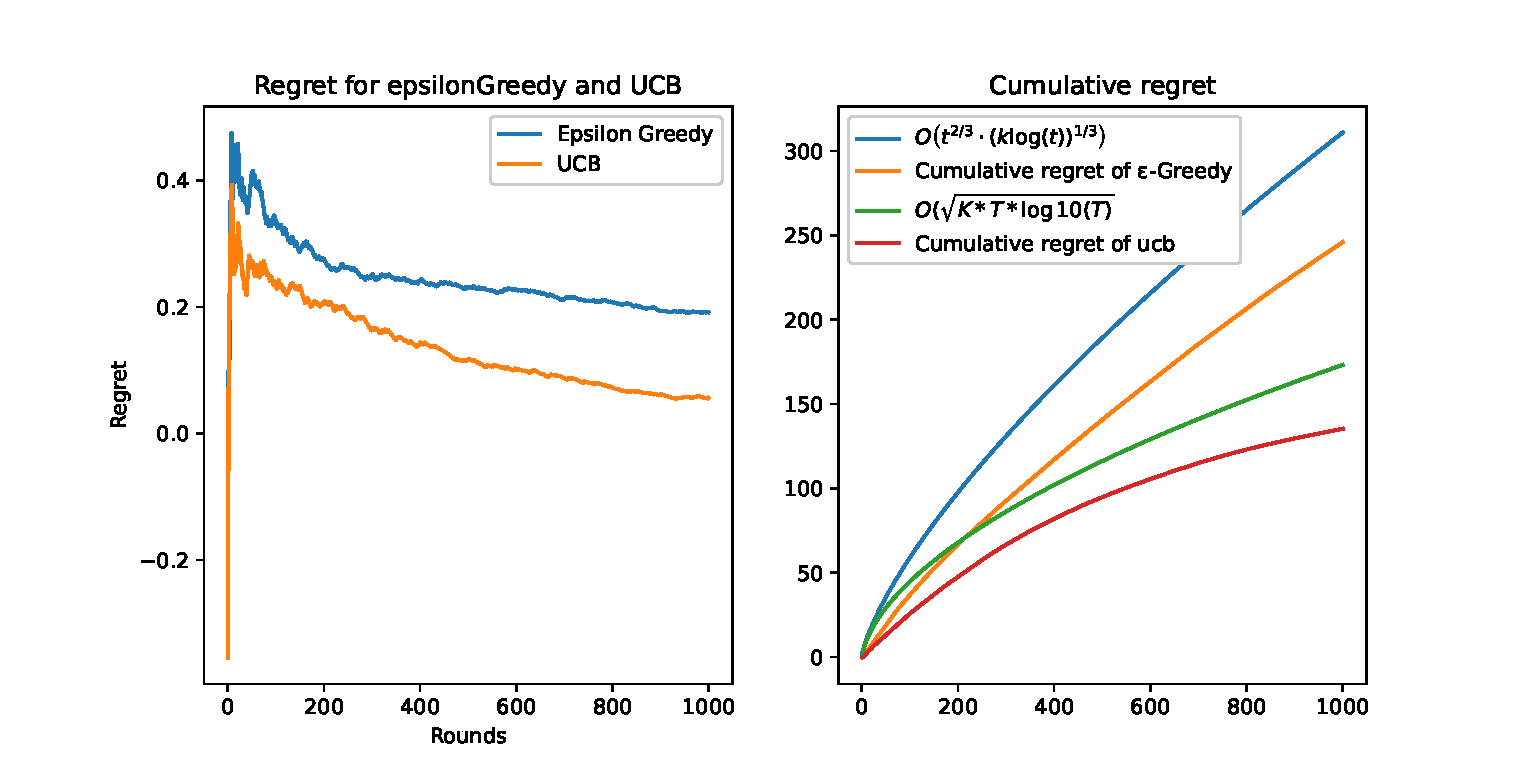
\includegraphics[width=1\linewidth]{Images/Regret10_1000_UCB.eps}
	  \captionof{figure}{Lower regret for UCB (K=10 T=1000)}
	  \label{fig:UCB_1000}
	\end{minipage}%
	\begin{minipage}{.5\textwidth}
		\centering
		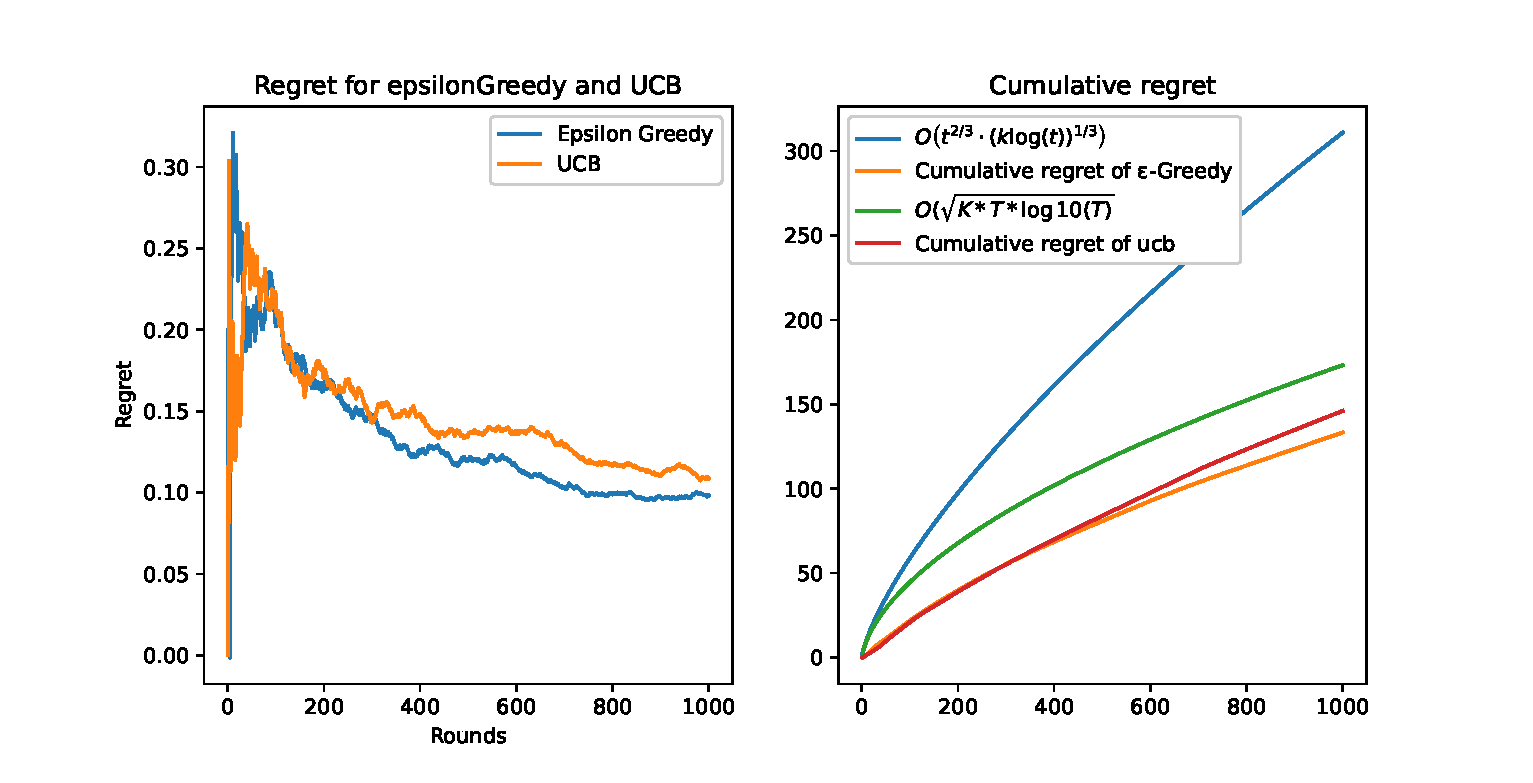
\includegraphics[width=1\linewidth]{Images/Regret10_1000_epsilon.eps}
		\captionof{figure}{Lower regret for ε-Greedy (K=10 T=1000)}
		\label{fig:epsilon_1000}
	\end{minipage}
\end{figure}
\clearpage

\noindent
Παρατηρώντας και το cumulative regret, στην σύγκριση μεταξύ των 2 αλγορίθμων τα αποτελέσματα είναι αναμενόμενα, τα αποτελέσματα είναι αναμενόμενα όπως και στην σύγκριση κάθε αλγόριθμου με το θεωρητικό του convergence rate. Το θεωρητικό convergence rate αποτελεί πάνω όριο εφόσον εμπεριέχονται τυχαίες μεταβλητές και όπως ήταν αναμενόμενο η γραφική του είναι πιο πάνω σε σχέση με τα πειραματικά δεδομένα.

\noindent\\
Για την καλύτερη επαλήθευση της εκτίμησης, αυξήθηκε η τιμή ορίζοντα (Τ = 10000) ενώ ο αριθμός των bandit παρέμεινε σταθερός (Κ = 10). Στην περίπτωση αυτή ο UCB πάντα παρουσιάζει καλύτερη επίδοση, δηλαδή μικρότερο regret, σε σχέση με τον ε-Greedy κάτι το οποίο επιβεβαιώνει την αρχική εκτίμηση. 


\begin{figure}[h]
	\centering
	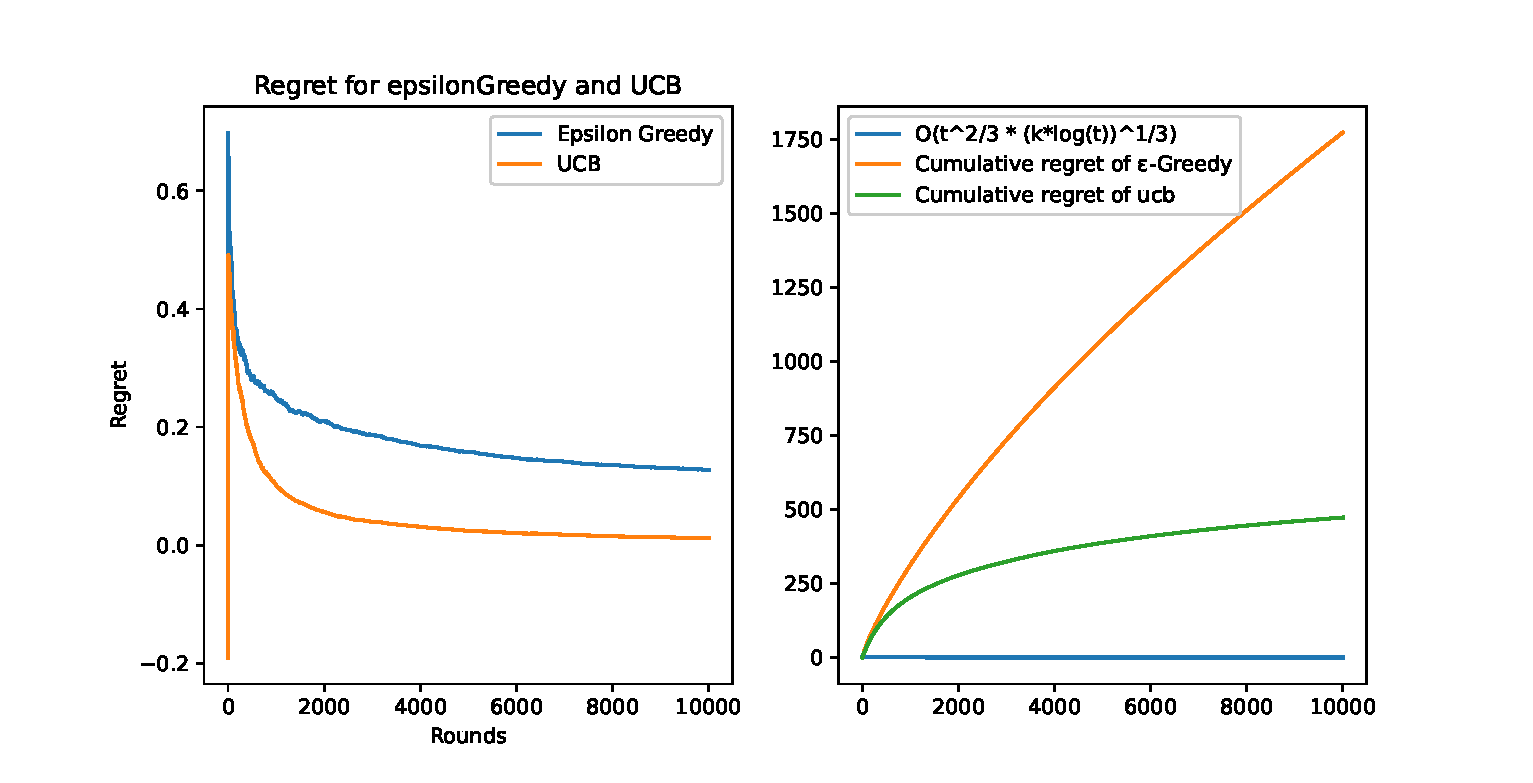
\includegraphics[width=.6\linewidth]{Images/Regret10_10000.eps} 
	\captionof{figure}{Lower regret for ε-Greedy (K=10 T=10000)} 
	\label{fig:epsilon_10000}
\end{figure}


\noindent
Παρατηρώντας συνολικά τις γραφικές, είναι εμφανές πως όσο αυξάνεται ο αριθμός των γύρων τόσο μειώνεται το regret αλλά και πως όσο αυξάνονται οι γύροι, o ρυθμός αύξησης του του regret μειώνεται και για του δύο αλγορίθμους κάτι το οποίο σημαίνει πως και οι δύο αλγόριθμοι επιτυγχάνουν sublinear πολυπλοκότητα δεδομένου του οτι ο ρυθμός αύξησης του regret μειώνεται όσο αυξάνονται οι γύροι.

\noindent\\
Τέλος, έγινε μεταβολή του αριθμού των bandits και πιο συγκεκριμένα τέθηκαν ίσοι με 5 και 20, για ορίζοντα 1000 και 10000 αντίστοιχα. Όπως ήταν αναμενόμενο στις περιπτώσεις που μειώνεται ο αριθμός των bandits, το regret σταθεροποιείται σε μικρότερη τιμή, ενώ αντίθετα αυξάνοντας τον αριθμό των bandits, αυξάνεται η τιμή σταθεροποίησης.


\begin{figure}[h]
	\centering
	\begin{minipage}{.4\textwidth}
	  \centering
	  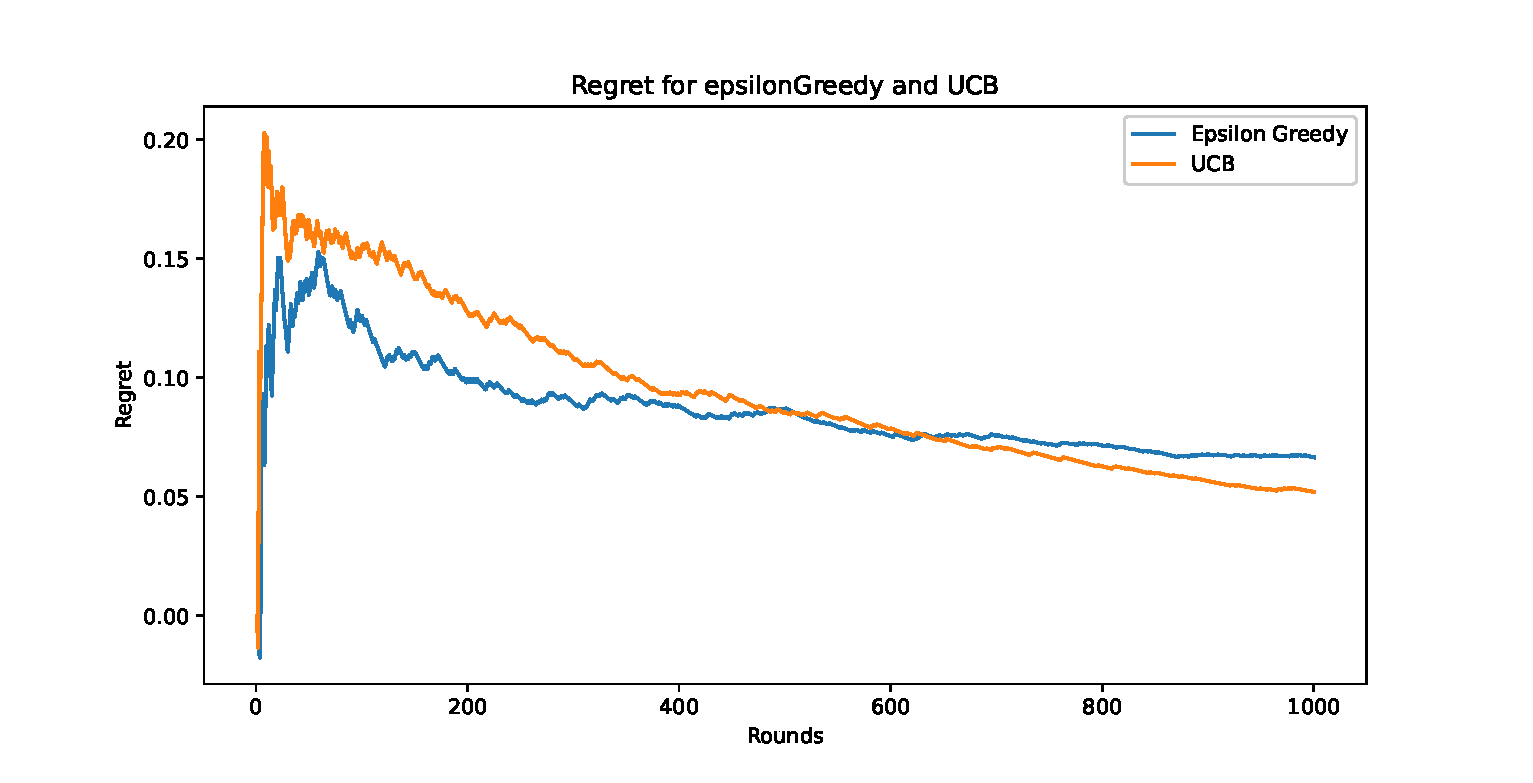
\includegraphics[width=0.9\linewidth]{Images/Regret5_1000.eps}
	  \captionof{figure}{K = 5, T = 1000}
	  \label{fig:UCB_13000}
	\end{minipage}%
	\begin{minipage}{.4\textwidth}
		\centering
		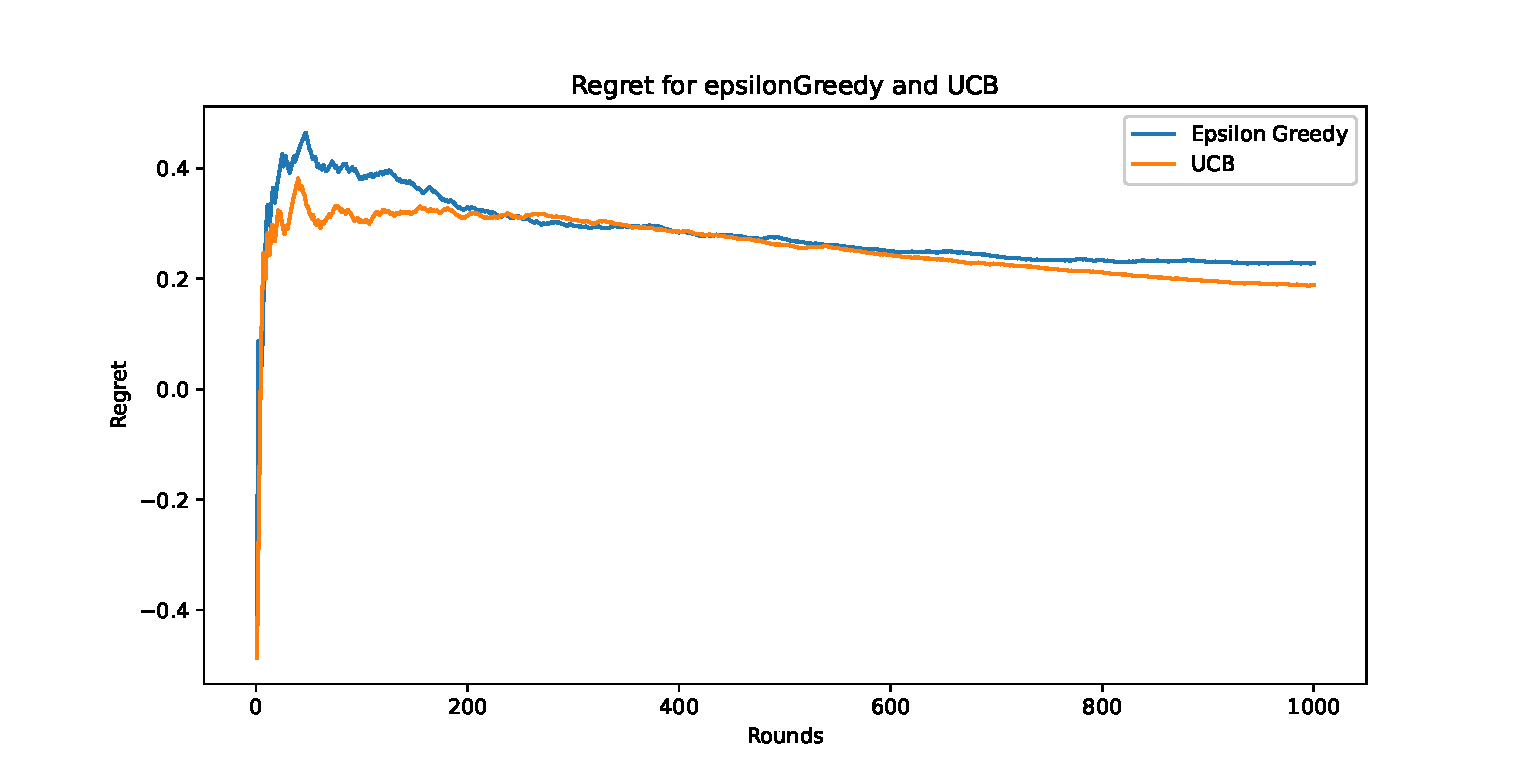
\includegraphics[width=0.9\linewidth]{Images/Regret20_1000.eps}
		\captionof{figure}{K = 20, T = 1000}
		\label{fig:epsilon_10020}
	\end{minipage}
\end{figure}

\begin{figure}[h]
	\centering
	\begin{minipage}{.4\textwidth}
		\centering
		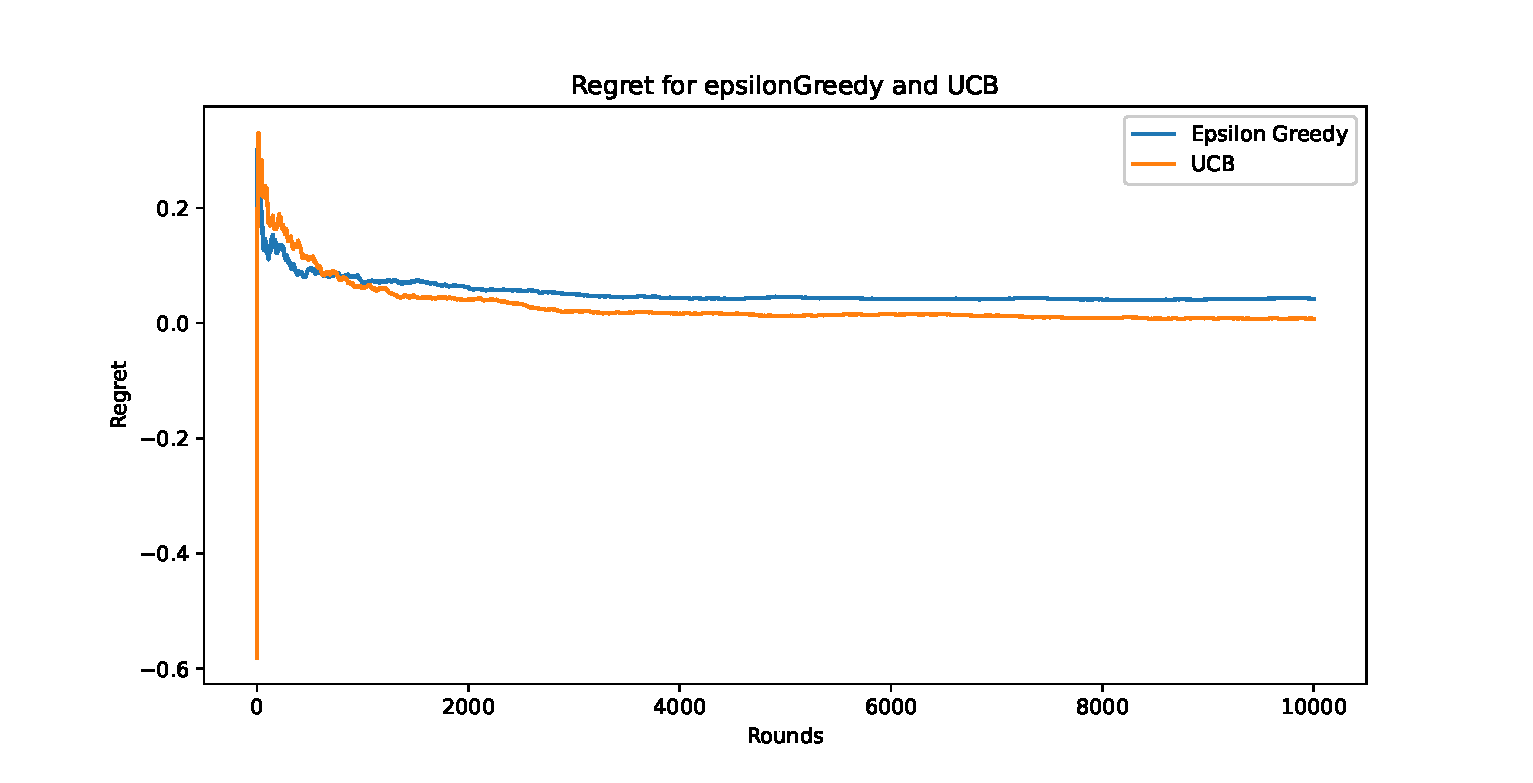
\includegraphics[width=0.9\linewidth]{Images/Regret5_10000.eps}
		\captionof{figure}{K = 5, T = 10000}
		\label{fig:epsilon_10001}
	\end{minipage}
	\begin{minipage}{.4\textwidth}
		\centering
		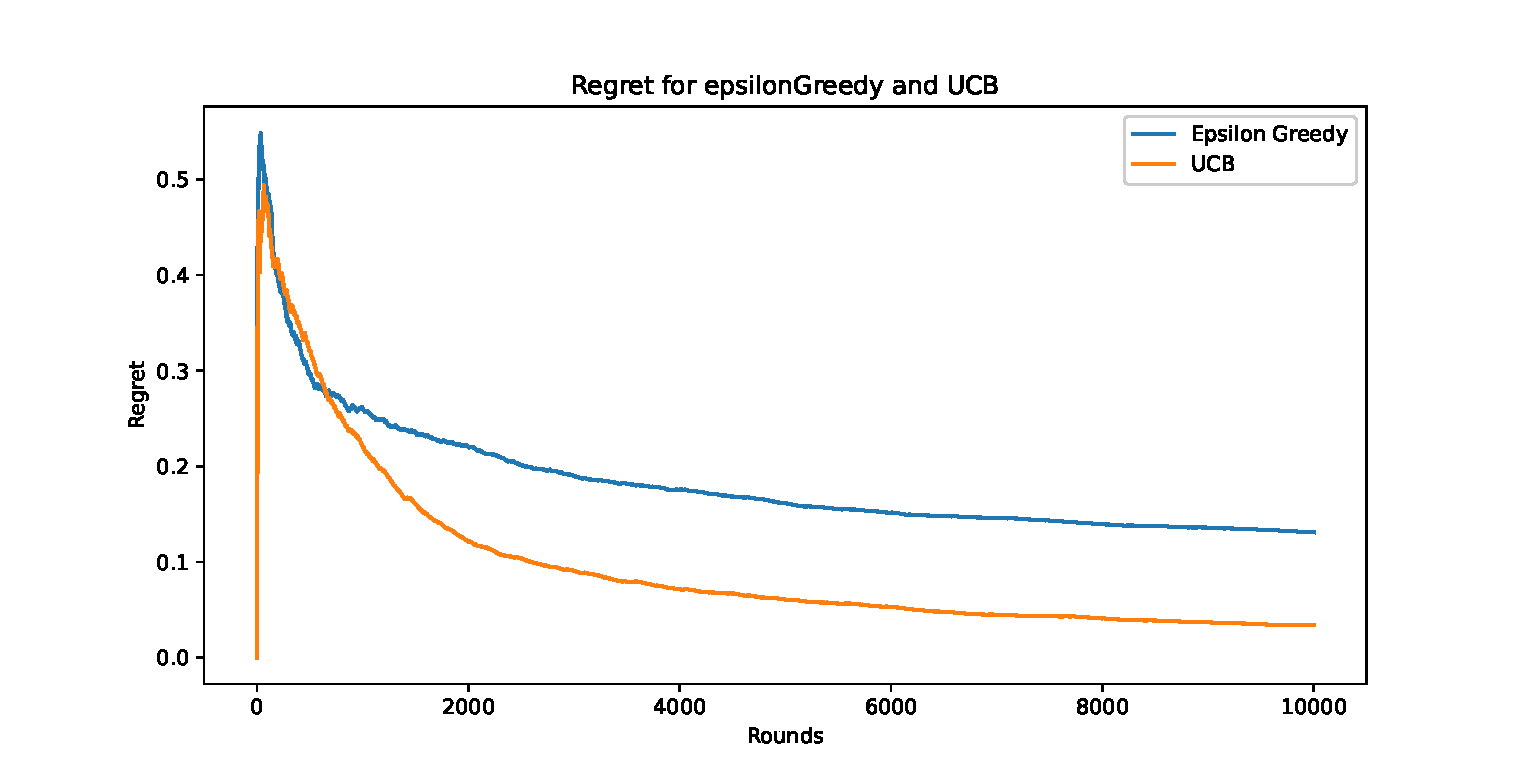
\includegraphics[width=0.9\linewidth]{Images/Regret20_10000.eps}
		\captionof{figure}{K = 20, T = 10000}
		\label{fig:epsilon_15000}
	\end{minipage}
\end{figure}

\noindent
Είναι αναμενόμενο και πάλι πως όσο αυξάνεται ο αριθμος των bandits το regret αυξάνεται και αντίστοιχα πως όσο αυξάνεται ο αριθμός των γύρων το regret μειώνεται.